\begin{figure}[!ht]
    \centering
    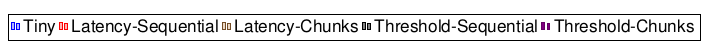
\includegraphics[scale=0.3]{images/legend}

    \subfloat[Tempo de execução]{
        \label{Yada}
        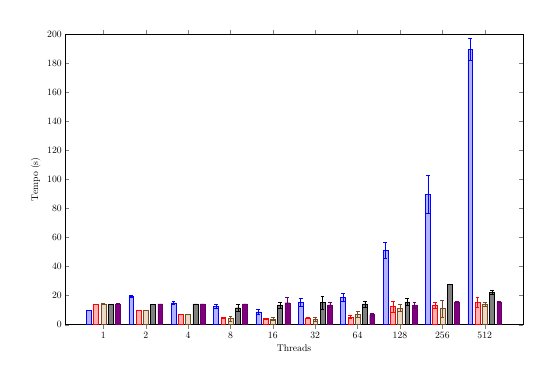
\begin{tikzpicture}[scale=0.35, baseline]
        \begin{axis}[
            width=1.5 \linewidth,
            height=1 \linewidth,
            %media de tempo intruder
            ybar=2.5pt,
            %enlargelimits=0.10,
            % legend style={at={(0.45,1.1)}, anchor=south, legend columns=-1},
            ylabel=Tempo (s),
            xlabel=Threads,
            symbolic x coords={1, 2, 4, 8, 16, 32, 64, 128, 256, 512},
            xtick=data,
            ymin=0,
            ymax=200,
            bar width=5pt,
            % nodes near coords,
            nodes near coords align={vertical},
        ]
        \addplot+[error bars,y dir=both, y explicit] coordinates {
            (1,9.95)+-(1,0.09) (2,19.42)+-(2,0.50) (4,15.05)+-(4,1.07) (8,12.75)+-(8,1.30) (16,8.85)+-(16,1.90) (32,15.25)+-(32,2.69) (64,18.85)+-(64,2.74) (128,51.34)+-(128,5.50) (256,89.66)+-(256,12.90) (512,189.43)+-(512,7.63) 
        };
        \addplot+[error bars,y dir=both, y explicit] coordinates {
            (1,14.09)+-(1,0.09) (2,9.88)+-(2,0.04) (4,7.22)+-(4,0.04) (8,4.78)+-(8,0.29) (16,4.19)+-(16,0.35) (32,4.74)+-(32,0.50) (64,5.38)+-(64,1.21) (128,12.38)+-(128,3.72) (256,13.14)+-(256,2.01) (512,15.43)+-(512,3.54)
        };
        \addplot+[error bars,y dir=both, y explicit] coordinates {
            (1,14.31)+-(1,0.16) (2,9.98)+-(2,0.07) (4,7.23)+-(4,0.11) (8,4.19)+-(8,1.93) (16,3.85)+-(16,0.97) (32,3.96)+-(32,1.37) (64,7.11)+-(64,1.83) (128,11.47)+-(128,2.48) (256,11.12)+-(256,5.94) (512,14.17)+-(512,1.47)
        };
        \addplot+[error bars,y dir=both, y explicit] coordinates {
            (1,14.17)+-(1,0.05) (2,14.17)+-(2,0.11) (4,14.20)+-(4,0.08) (8,11.61)+-(8,2.13) (16,13.53)+-(16,1.93) (32,15.15)+-(32,4.48) (64,14.19)+-(64,2.00) (128,15.69)+-(128,2.21) (256,27.92)+-(256,0.20) (512,22.18)+-(512,1.28) 
        };
        \addplot+[error bars,y dir=both, y explicit] coordinates {
            (1,14.35)+-(1,0.05) (2,14.29)+-(2,0.04) (4,14.31)+-(4,0.08) (8,14.31)+-(8,0.05) (16,15.07)+-(16,4.06) (32,13.64)+-(32,1.83) (64,6.83)+-(64,1.09) (128,13.37)+-(128,2.19) (256,15.65)+-(256,0.16) (512,15.73)+-(512,0.14)
        };
        % \legend {Tiny, Latency-Sequential, Latency-Chunks, Threshold-Sequential, Threshold-Chunks}
        \end{axis}
        \end{tikzpicture}
    }
    \subfloat[Aborts]{
        \label{abortYada}
        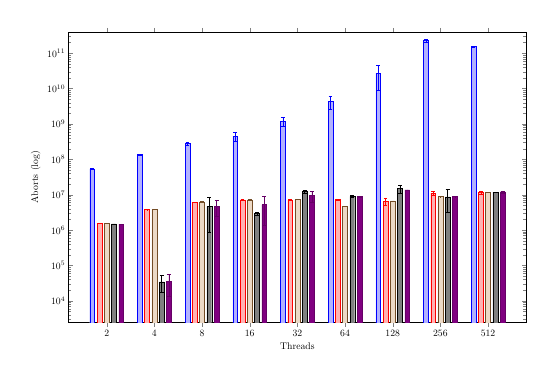
\begin{tikzpicture}[scale=0.35, baseline]
        \begin{axis}[
            ymode=log,
            width=1.5 \linewidth,
            height=1 \linewidth,
            %media de tempo intruder
            ybar=2.5pt,
            %enlargelimits=0.10,
            % legend style={at={(0.45,1.1)}, anchor=south, legend columns=-1},
            ylabel=Aborts (log),
            xlabel=Threads,
            symbolic x coords={1, 2, 4, 8, 16, 32, 64, 128, 256, 512},
            xtick=data,
            ymin=0,
            ymax=400000000000,
            bar width=5pt,
            % nodes near coords,
            nodes near coords align={vertical},
        ]
        \addplot+[error bars,y dir=both, y explicit] coordinates {
            (1,0.0)+-(1,0.0) (2,53805739.2)+-(2,945974.4856792702) (4,136025541.2)+-(4,4837342.13) (8,281305083.6)+-(8,28618515.67361887) (16,455944205.2)+-(16,138166587.07) (32,1205121875.2)+-(32,315403375.80832976) (64,4297295036.4)+-(64,1609418223.03) (128,27371816768.6)+-(128,18399453268.002537) (256,230017372308.6)+-(256,19982225506.96) (512,156775482845.2)+-(512,5418181512.20) 
        };
        \addplot+[error bars,y dir=both, y explicit] coordinates {
            (1,0.0)+-(1,0.0) (2,1580633.2)+-(2,8478.500749542929) (4,3800972.6)+-(4,20650.110223434644) (8,6149664.4)+-(8,75882.93103880476) (16,7207458.2)+-(16,106075.91092684522) (32,7097792.4)+-(32,149914.3555148739) (64,7245601.6)+-(64,297306.3815181907) (128,6626592.6)+-(128,1601916.1098185633) (256,11035923.666666666)+-(256,1354186.7993902795) (512,11463741.25)+-(512,1422857.6912357355)
        };
        \addplot+[error bars,y dir=both, y explicit] coordinates {
             (1,0.0)+-(1,0.0) (2,1586885.6)+-(2,17013.20809959133) (4,3864768.25)+-(4,23733.99245149244) (8,6283745.6)+-(8,79485.5) (16,7192878.4)+-(16,178424.65) (32,7378729.9)+-(32,18573.11) (64,4723078.0)+-(64,3928.0) (128,6736182.0)+-(128,37123.3) (256,8828877.0)+-(256,12847.0) (512,11637482.0)+-(512,82034.0) 
        };
        \addplot+[error bars,y dir=both, y explicit] coordinates {
            (1,0.0)+-(1,0.0) (2,1502389.8)+-(2,8336.5398735266599) (4,34570.6)+-(4,17081.853735470282) (8,4673390.0)+-(8,3789634.775837482) (16,2964970.8)+-(16,290439.4272928145) (32,12301780.8)+-(32,1054972.452489657) (64,9002166.4)+-(64,735560.767845634) (128,14938022.8)+-(128,3727246.128412794) (256,8642330.0)+-(256,5465830.0) (512,11928378.731)+-(512,74928.0)
        };
        \addplot+[error bars,y dir=both, y explicit] coordinates {
            (1,0.0)+-(1,0.0) (2,1483981.3)+-(2,5287.71) (4,34983.38)+-(4,21305.7) (8,4728374.12)+-(8,2263748.1) (16,5260517.0)+-(16,3862894.25) (32,9462941.0)+-(32,3192100.38) (64,8837692.27)+-(64,384722.0) (128,13729279.5)+-(128,110344.5) (256,8874348.23)+-(256,63743.0) (512,11973628.0)+-(512,837874.02)
        };
        % \legend {Tiny, Latency-Sequential, Latency-Chunks, Threshold-Sequential, Threshold-Chunks}
        \end{axis}
        \end{tikzpicture}
    }
\end{figure}
